\documentclass{beamer}
\usepackage[spanish]{babel}
\usepackage[utf8]{inputenc}
\usepackage{graphicx}
\usepackage{multimedia}
\usepackage{animate}
\usebackgroundtemplate{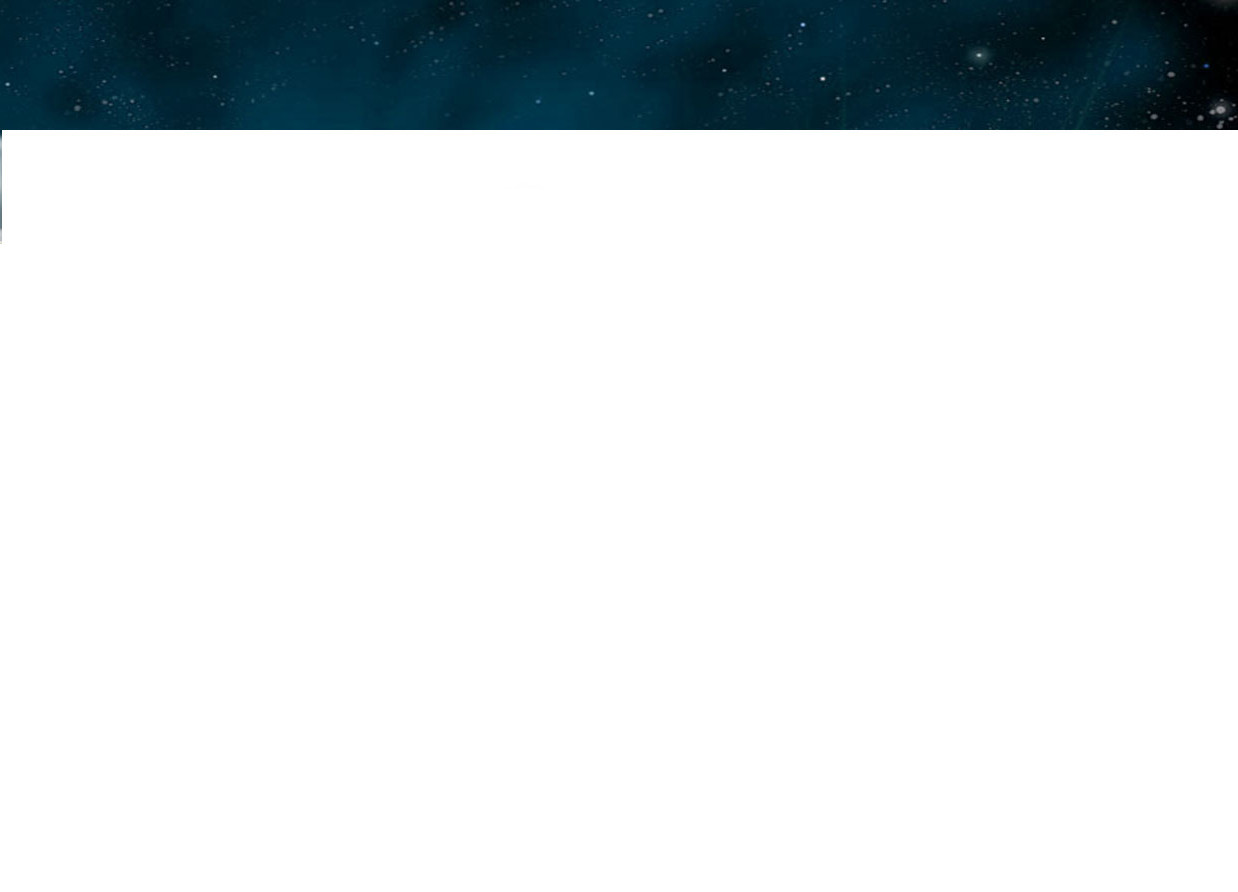
\includegraphics[width=\paperwidth]{sources/images/template_internal.jpg}}
\setbeamercolor{frametitle}{fg=white}
\usefonttheme{structuresmallcapsserif}
\setbeamertemplate{footline}[frame number]

\usepackage{default}

\newcounter{stepsBarnes}
\newcommand{\seti}{\setcounter{stepsBarnes}{\value{enumi}}}
\newcommand{\conti}{\setcounter{enumi}{\value{stepsBarnes}}}
\definecolor{green}{RGB}{0, 150, 0}

\begin{document}
{
	\usebackgroundtemplate{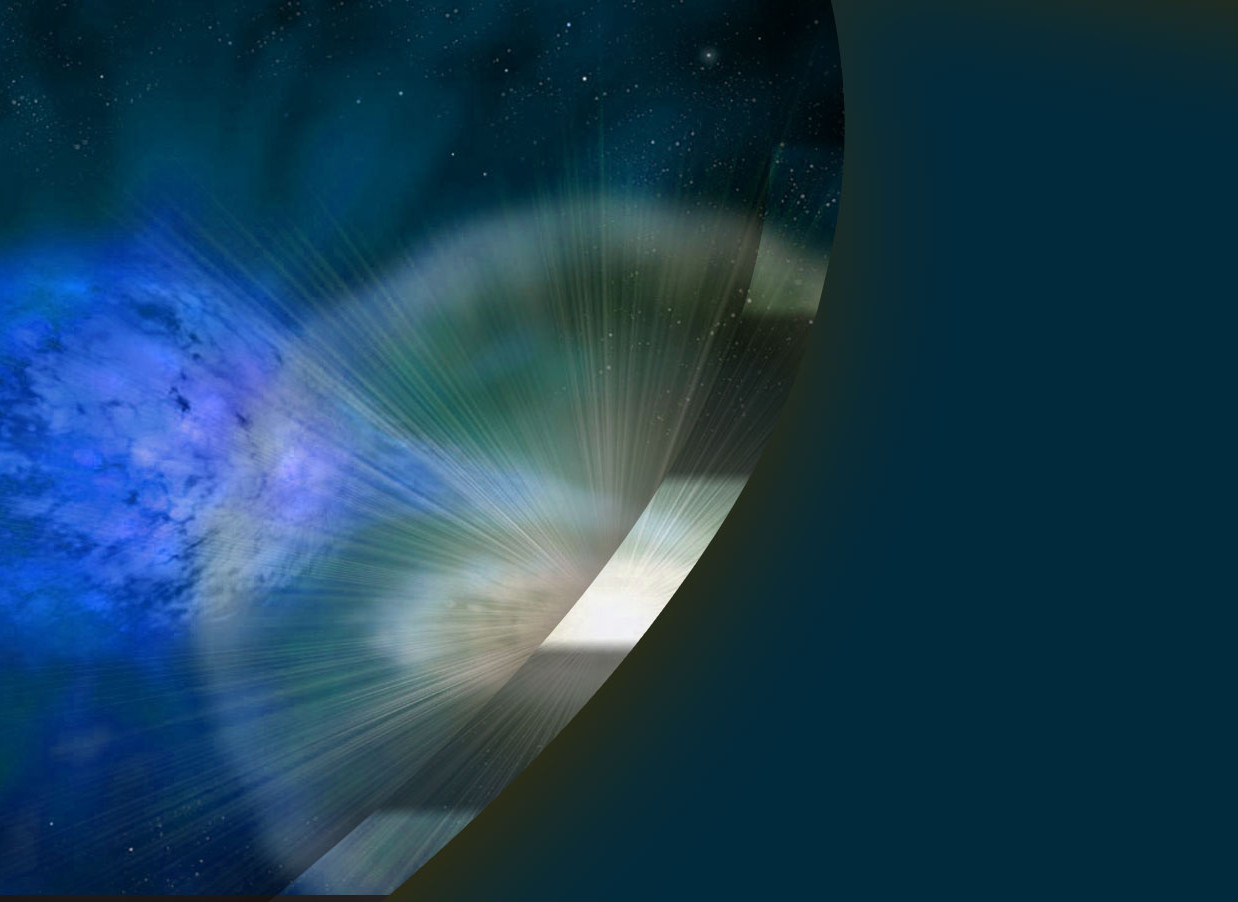
\includegraphics[width=\paperwidth]{sources/images/template_main.jpg}}
	\begin{frame}
		\centering
		\color{white}
		\textsc{\LARGE Dinámica de galaxias, una simulación con $N\log N$ iteraciones.}
		\\
		\vspace{5cm}
		\raggedleft Juan Barbosa
	\end{frame}
}

\begin{frame}{Introducci\'on}
	\centering
	\begin{columns}
		\begin{column}{.5\textwidth}
			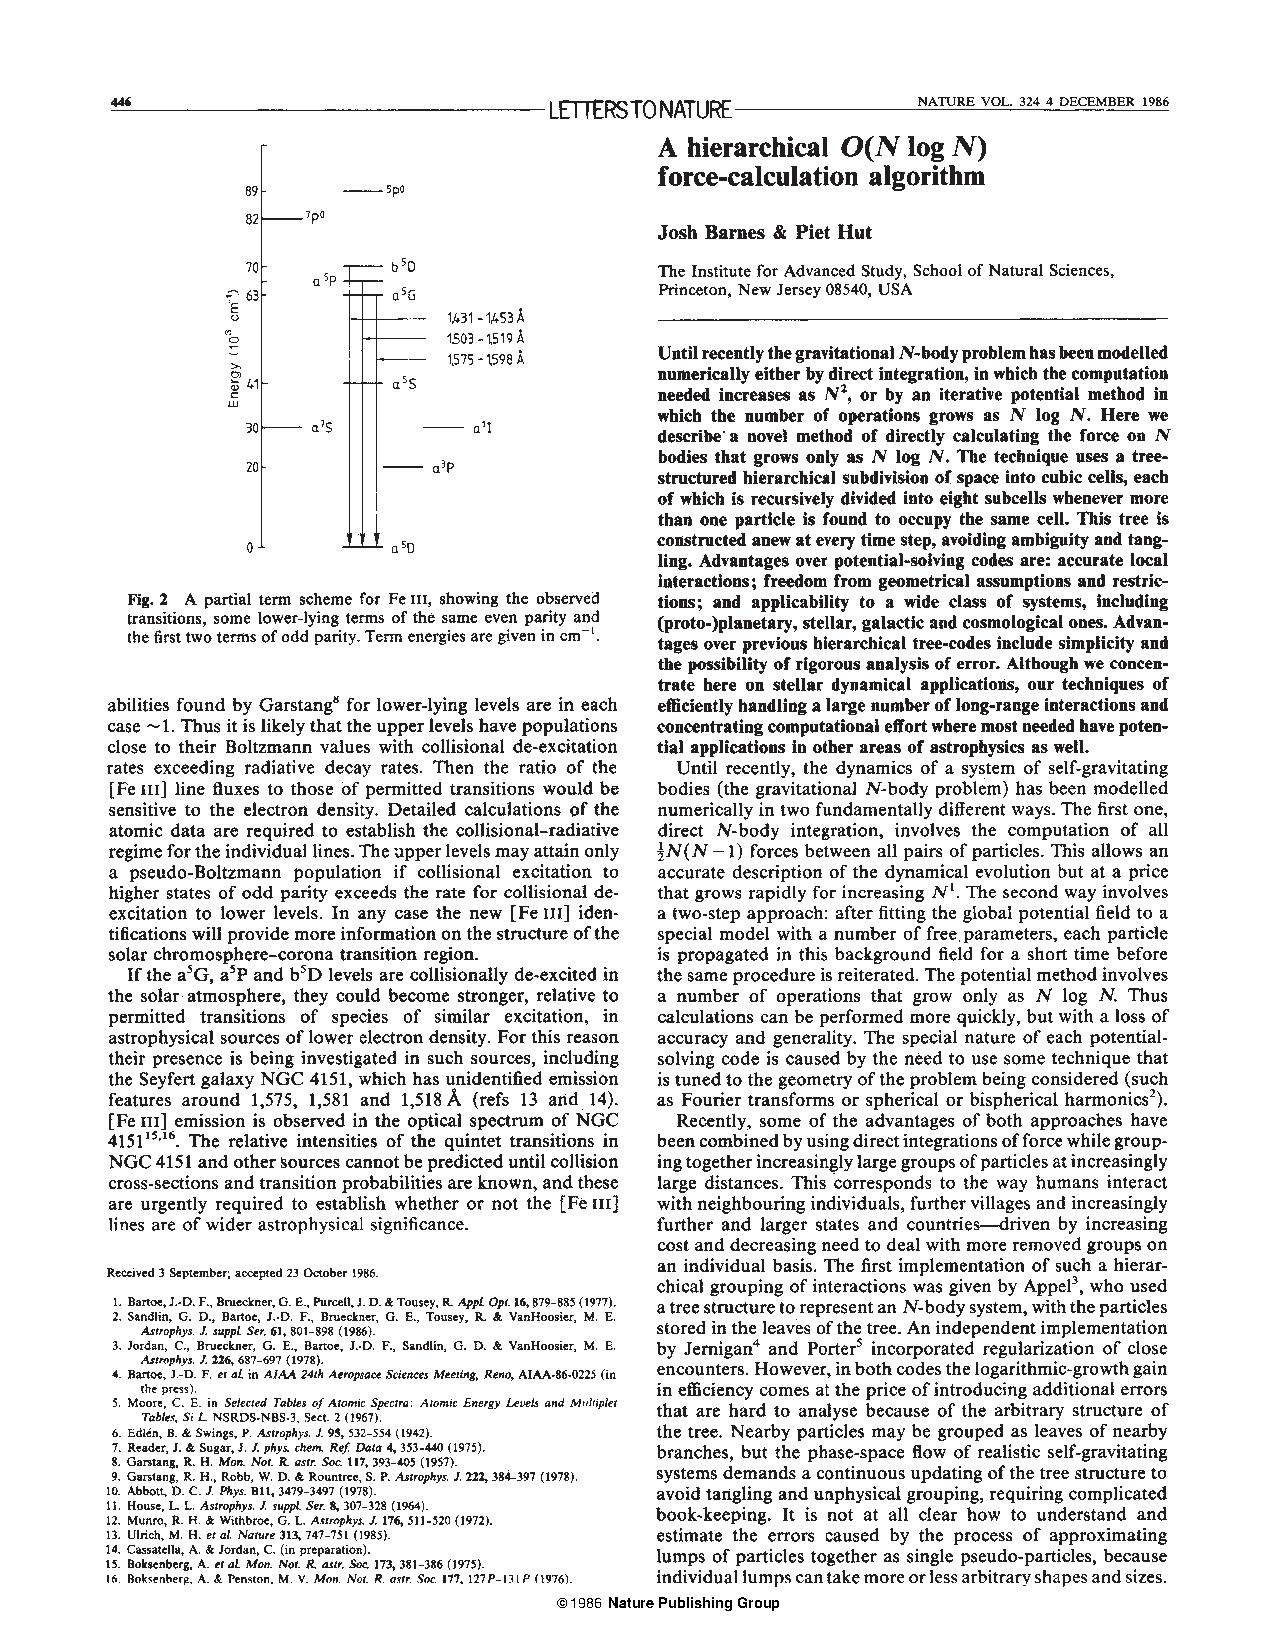
\includegraphics[height=0.8\textheight]{sources/images/barnes1986.pdf}
		\end{column}
		\begin{column}{.5\textwidth}
			\centering
			\begin{tabular}{cc}
				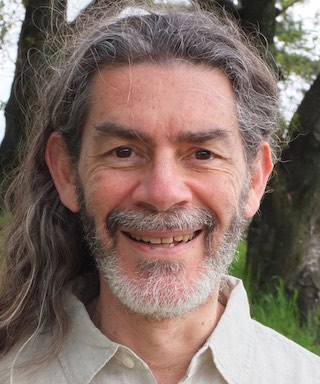
\includegraphics[height=0.3\textheight]{sources/images/barnes.jpg} & Josh Barnes\\
				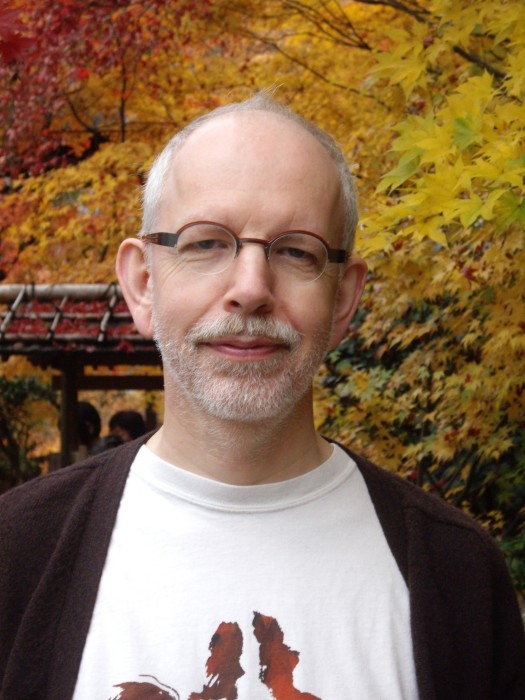
\includegraphics[height=0.3\textheight]{sources/images/hut.jpg}
				& Piet Hut \\
			\end{tabular}
		\end{column}
	\end{columns}
	
\end{frame}

\begin{frame}{Introducci\'on}
	\begin{columns}
		\begin{column}{.5\textwidth}
			\begin{tabular}{c}
				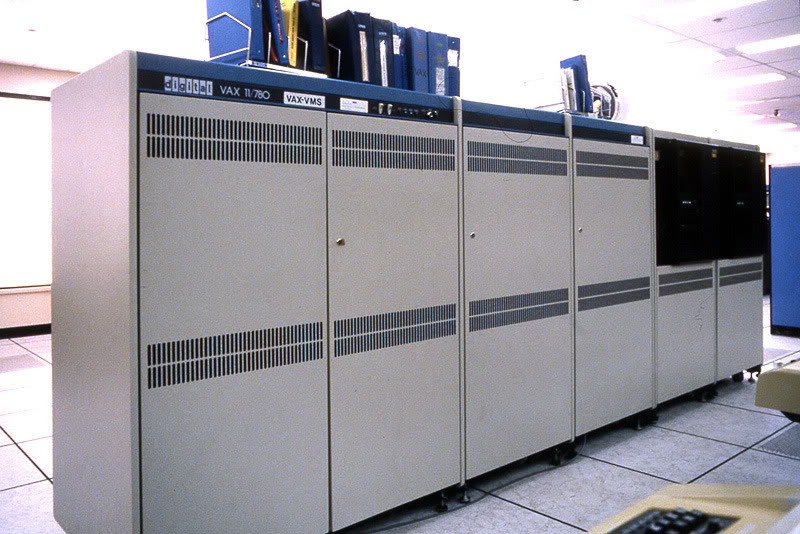
\includegraphics[width=\textwidth]{sources/images/DEC-VAX-11-780} \\
				VAX 11/780
			\end{tabular}
		\end{column}
		\begin{column}{.5\textwidth}
			\begin{itemize}
				\item<2-> Simulaci\'on con 4096 cuerpos.
				\item<3-> Tiempo: 10 horas de CPU.
			\end{itemize}
		\end{column}
	\end{columns}
\end{frame}
\begin{frame}{Funcionamiento}
	El algoritmo propuesto por Barnes y Hut consta de dos pasos fundamentales, la divisi\'on recursiva del espacio y la forma como se calcula la fuerza sobre un cuerpo. \pause
	\begin{enumerate}
		\item Divisi\'on jer\'arquica del espacio. \pause
		\seti
	\end{enumerate}
	\begin{columns}
		\begin{column}{0.5\linewidth}
			\centering
			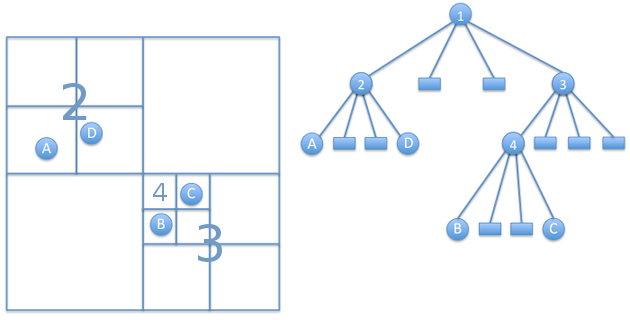
\includegraphics[width=\linewidth]{sources/images/quadtree.png}\\
			\'Arbol dos dimensional.\pause
		\end{column}
		\begin{column}{0.5\linewidth}
			\centering
			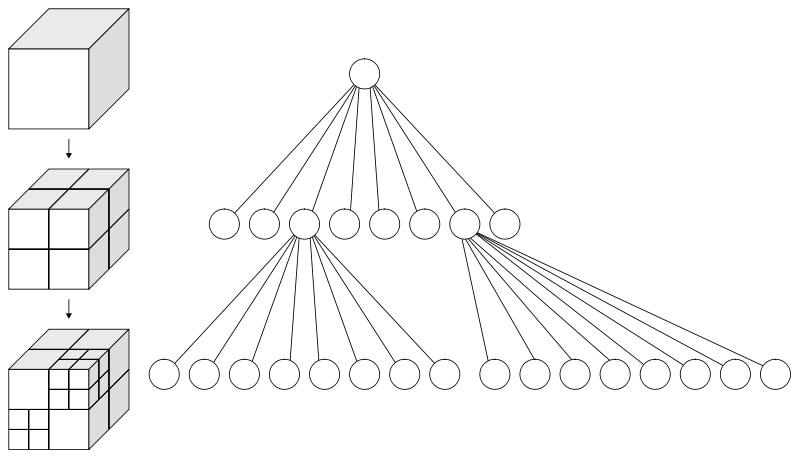
\includegraphics[width=\linewidth]{sources/images/octree.png}\\
			\'Arbol tridimensional.
		\end{column}
	\end{columns}
\end{frame}
\begin{frame}{Funcionamiento}
	\begin{enumerate}
		\conti
		\item Fuerza sobre un cuerpo.
	\end{enumerate}
	\small
	El n\'umero de iteraciones se reduce al considerar centros de masa y distancias. \pause
	\begin{itemize}
		\item Cada caja tiene una longitud espec\'ifica \pause
		\item Un centro de masa \pause
		\item Y la masa contenida \pause
	\end{itemize}
	\centering
	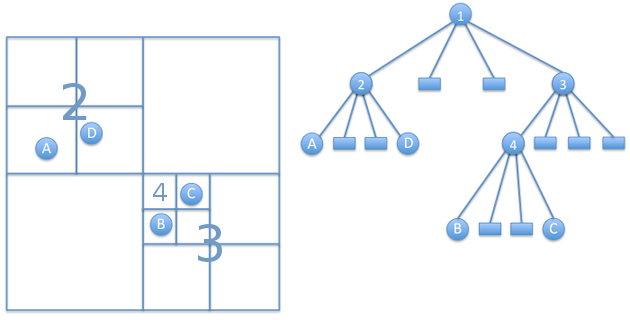
\includegraphics[width=0.5\linewidth]{sources/images/quadtree.png}
\end{frame}
\begin{frame}{Funcionamiento}
	\begin{columns}
		\begin{column}{0.6\textwidth}
			\centering
			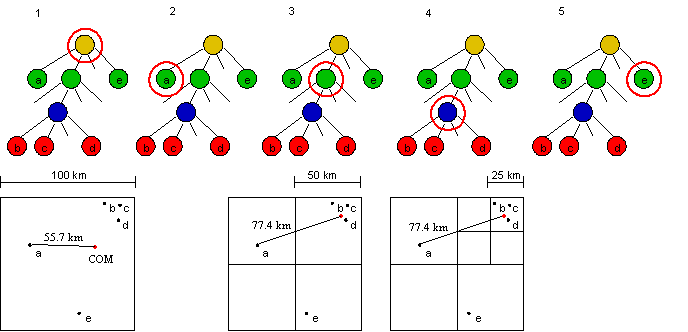
\includegraphics[width=\linewidth]{sources/images/force.png}\\
			\begin{itemize}
				\item Se define un coeficiente de precisi\'on.
			\end{itemize}
			$\theta = 0.5$
			\pause
		\vspace{1cm}
		
		\end{column}
		\begin{column}{0.4\textwidth}
			\begin{enumerate}
				\footnotesize
				\item {\color{orange} Nodo principal} \pause
				\begin{equation*}
					\dfrac{s}{d} = \dfrac{100}{55.7} \approx 1.8 > \theta 
				\end{equation*}
				\pause
				\item {\color{green} Primer nodo} \pause
				\item {\color{green} Segundo nodo} \pause
				\begin{equation*}
					\dfrac{s}{d} = \dfrac{50}{77.4} \approx 0.6 > \theta 
				\end{equation*}
				\pause
				\item {\color{blue} Segundo nodo} \pause
				\boxed{\dfrac{s}{d} = \dfrac{25}{77.4} \approx 0.3 < \theta}
				\pause
				\item {\color{green} Cuarto nodo} \pause
				\boxed{\text{Nodo externo, contribuye}}
			\end{enumerate}
		\end{column}
	\end{columns}
\end{frame}
\begin{frame}{Funcionamiento}
	La construcci\'on del arbol se realiza para cada instante de tiempo.
	\centering
	\movie[height = 0.55\textwidth, width = 0.8\textwidth, poster, showcontrols]{}{sources/animations/boxes_points.mp4}
	\\
	Observaci\'on
\end{frame}
\begin{frame}{Funcionamiento}
	La construcci\'on del arbol se realiza para cada instante de tiempo.
	\centering
	\movie[height = 0.55\textwidth, width = 0.8\textwidth,poster, showcontrols]{}{sources/animations/boxes.mp4}
	\\
	Todas las cajas
\end{frame}
\begin{frame}{Funcionamiento}
	La construcci\'on del arbol se realiza para cada instante de tiempo.
	\centering
	\movie[height = 0.55\textwidth, width = 0.8\textwidth, poster, showcontrols]{}{sources/animations/boxes_child_only.mp4}
	\\
	Cajas con una part\'icula
\end{frame}
\begin{frame}{Construcci\'on de una simulaci\'on}
	\begin{enumerate}
		\item Descripci\'on del sistema. \pause
		\item Condiciones iniciales. \pause
		\item Soluci\'on de las ecuaciones. \pause
		\item Visualizaci\'on.
	\end{enumerate}
\end{frame}
\begin{frame}{Descripci\'on del sistema}
	Usando la ley de gravitaci\'on universal:
	\begin{equation}
		\vec{F_i} = m_i\vec{a}_i = - \sum\limits_{j\neq i}^N G\dfrac{m_im_j}{|\vec{r}_{ij}|^3}\left(\vec{r}_i - \vec{r}_j\right)
	\end{equation}\pause
	es posible obtener las ecuaciones que describen la din\'amica del sistema.\pause
	\begin{equation}
		\vec{\ddot{r}}_i = - \sum\limits_{j\neq i}^N G\dfrac{m_j}{|\vec{r}_{ij}|^3}\left(\vec{r}_i - \vec{r}_j\right)
	\end{equation}
\end{frame}
\begin{frame}{Condiciones iniciales}
	Suponiendo \'orbitas circulares y teniendo en cuenta la masa encerrada en las \'orbitas de menor tama\~no:
	\begin{equation}
		v \approx \sqrt{\dfrac{GM(r)}{r}}
	\end{equation}
	
	En coordenadas polares:
	\begin{equation}
		\begin{matrix}
			x = r\cos(\theta) \qquad \longrightarrow \qquad \dot{x} = -r\sin(\theta) = -y \\
			y = r\sin(\theta) \qquad \longrightarrow \qquad \dot{y} = r\cos(\theta) = x
		\end{matrix}
	\end{equation}
\end{frame}

\end{document}